\documentclass[12pt,a4paper]{article}
\usepackage[margin=1in]{geometry}
\usepackage{setspace}
\usepackage{graphicx}
\usepackage{amsmath, amssymb}
\usepackage{booktabs}
\usepackage{longtable}
\usepackage{caption}
\usepackage{float}
\usepackage{hyperref}
\usepackage{pgfgantt}
\usepackage{tikz}
\usetikzlibrary{shapes.geometric, arrows.meta, positioning}
\usepackage{enumitem}
\usepackage{array}
\usepackage{multirow}
\usepackage{natbib}
\usepackage{url}
\usepackage{xcolor}
\setlength{\parindent}{0pt}
\setlength{\parskip}{6pt}

\title{\textbf{Predicting Inland Waterway Navigability\\Using Satellite Remote Sensing and Machine Learning}}
\author{}
\date{}

\begin{document}

\maketitle

\vspace{-1cm}
\begin{center}
\begin{tabular}{ccc}
\textbf{Dev Yadav} & \textbf{Chakshu Vashisth} & \textbf{Ankit Gupta} \\
{\small UG Student} & {\small UG Student} & {\small UG Student} \\
{\small Gati Shakti Vishwavidyalaya,} & {\small Gati Shakti Vishwavidyalaya,} & {\small Gati Shakti Vishwavidyalaya,} \\
{\small Vadodara, India - 390004} & {\small Vadodara, India - 390004} & {\small Vadodara, India - 390004} \\
\end{tabular}
\end{center}

\vspace{0.3cm}
\onehalfspacing

%==============================================================
\section*{1. Origin of the Proposal}
%==============================================================

India possesses roughly 14,500 kilometres of rivers and canals that could serve freight and passenger movement, yet barely 2\% of this network carries any meaningful cargo today. In contrast, waterway freight accounts for 44\% of total cargo in the European Union and about 25\% in the United States, revealing a massive gap in utilisation. Recognising this, the Government of India enacted the National Waterways Act in 2016, declaring 111 rivers and canal stretches as National Waterways (NWs), and committed over INR 5,000 crore under the Jal Marg Vikas Project (JMVP) to upgrade NW-1 along the Ganga alone.

A persistent bottleneck, however, is \textit{navigability assessment}. Before vessels can operate on any stretch, channel depth, width, and flow conditions must meet minimum thresholds, typically 2.5 to 3.0 metres of Least Available Depth (LAD) for standard 1,500 DWT barges. At present, the Inland Waterways Authority of India (IWAI) conducts monthly longitudinal surveys using echo sounders mounted on boats, a process that is labour intensive, costly, and covers only small segments at a time. Large portions of the 111 declared waterways remain unsurveyed, leaving planners with incomplete information on seasonal usability.

Satellite remote sensing offers a scalable alternative. Freely available multispectral imagery from the European Space Agency's Sentinel-2 constellation provides 10-metre spatial resolution every five days, capturing spectral signatures that correlate with water depth, turbidity, and surface extent. When combined with supervised machine learning models trained on sparse ground-truth depth readings from the Central Water Commission (CWC), it becomes feasible to generate continuous depth and navigability estimates over hundreds of kilometres, across multiple seasons, without deploying survey boats.

This project proposes to develop a data-driven framework that fuses multi-temporal Sentinel-2 imagery with hydrological gauge data and topographic information to predict navigability conditions on selected National Waterways. The system will classify each river segment as navigable, conditionally navigable, or non-navigable for a given month, and produce seasonal navigability calendars that support route planning and infrastructure investment decisions by IWAI and logistics operators.

\newpage
%==============================================================
\section*{2. Review of Status of Research and Development in the Subject}
%==============================================================

\subsection*{2.1 International Status}

Research at the intersection of satellite remote sensing and inland water depth estimation has progressed considerably over the past decade, driven by the availability of open-access satellite archives and advances in machine learning.

\textbf{1. Satellite Derived Bathymetry (SDB)}

The foundational work on estimating water depth from optical imagery dates back to Lyzenga (1978, 1985), who showed that the logarithm of water-leaving radiance in the visible bands decays linearly with depth in optically shallow water. Stumpf \textit{et al.} (2003) simplified this into a band-ratio approach using the natural log of blue and green reflectance, making it applicable to multispectral sensors without detailed knowledge of bottom substrates. These empirical models remain widely used baselines. More recently, Caballero and Stumpf (2020) demonstrated that the band-ratio model works reliably with Sentinel-2 data for depths up to 20 metres in clear water, achieving root mean square errors (RMSE) below 1.5 metres in Mediterranean coastal zones.



\textbf{2. Machine Learning for Depth Estimation}

Ensemble tree methods have emerged as the dominant approach for satellite-based bathymetry regression. A 2023 study by Li \textit{et al.}, working with Sentinel-2 images over Ganquan Dao Island, compared Random Forest (RF), Support Vector Regression (SVR), Artificial Neural Networks (ANN), and the Stumpf empirical model. Random Forest achieved the highest accuracy with an $R^{2}$ of 0.96 and RMSE of 1.41 m on test data, outperforming SVR ($R^{2}$ = 0.91) and ANN ($R^{2}$ = 0.88). The study attributed RF's advantage to its ability to handle non-linear spectral-depth relationships and its robustness against overfitting. Meanwhile, a 2025 preprint by Zhang \textit{et al.} evaluated a spectral-geospatial variant of XGBoost (SG-XGBoost) on the turbid Sancha Lake, reporting RMSE of 1.44 m, which outperformed standard RF (RMSE = 1.98 m) in the same setting. This finding underlines the value of incorporating spatial context when operating in optically complex waters.

Fine Decision Tree (FDT) regressors have also shown promise for river environments specifically. Hassan \textit{et al.} (2023) applied FDT to multispectral imagery from a section of the Nile, obtaining $R^{2}$ of 0.86 and RMSE of 2.09 m in waters up to 15 metres deep, a range that covers most Indian inland navigation channels.

\textbf{3. Water Surface Monitoring with Spectral Indices}

The Normalized Difference Water Index (NDWI), proposed by McFeeters (1996), and its Modified variant (MNDWI) by Xu (2006) are the workhorses of satellite-based water extent mapping. These indices exploit the contrast between green and near-infrared (or shortwave infrared) reflectance to segment water pixels from land. Chen \textit{et al.} (2023) used time series of MNDWI computed from Sentinel-2 over the Aral Sea Basin rivers between 2017 and 2022, revealing that river widths vary by up to 40\% between the warm and cold seasons. Such temporal analysis is directly transferable to Indian rivers, where monsoon-driven discharge fluctuations can be even more extreme.

\textbf{4. Hydrodynamic Modelling Augmented by Satellite Data}

Beyond depth estimation, several groups have used satellite altimetry (from missions such as Jason-3 and Sentinel-6) to calibrate and validate one-dimensional hydrodynamic models (HEC-RAS, MIKE 11) for large rivers. Papa \textit{et al.} (2022) combined multi-mission altimetry with the LISFLOOD-FP model on the Mahanadi River in India, creating a virtual stage-discharge network for stretches that lack physical gauges. The Surface Water and Ocean Topography (SWOT) mission, launched in December 2022, now provides two-dimensional water surface elevation maps at roughly 100-metre resolution, which can feed directly into hydraulic models predicting channel velocity and depth profiles.

\textbf{5. Vessel Detection and Traffic Monitoring}

Complementing the physical channel assessment, deep learning has been applied to detect and characterise vessels on inland waterways from satellite imagery. YOLO-family architectures fused with Automatic Identification System (AIS) transponder data have achieved detection accuracies exceeding 90\% on Rhine and Danube segments, as reported by Wu \textit{et al.} (2024). Such vessel intelligence can be combined with navigability maps to optimise scheduling and route planning.

\vspace{0.3cm}
Taken together, the international literature demonstrates that the components required for a navigability prediction system, including depth estimation, water extent monitoring, seasonal trend analysis, and vessel tracking, have individually reached high maturity levels. However, no study has \textit{integrated} these components into a unified pipeline tailored for inland navigation corridor assessment, and very few have addressed tropical monsoon-fed rivers, leaving a clear research gap this project aims to fill.

\newpage
\subsection*{2.2 National Status}

Indian contributions in this domain span government-led programmes, space agency initiatives, and academic research, though dedicated work on waterway navigability prediction remains sparse.

\textbf{1. ISRO and IIRS Initiatives}

The Indian Institute of Remote Sensing (IIRS, Dehradun), operating under the Department of Space, has led projects on estimating water levels in inland water bodies using multi-sensor satellite data. Researchers at IIRS developed algorithms combining radar altimetry from Saral/AltiKa and optical imagery from Resourcesat-2 to retrieve river stages along the Ganga, achieving agreement within 30 cm against CWC gauge readings (Dubey \textit{et al.}, 2020). In collaboration with IIT Roorkee, another IIRS group evaluated Jason-3 and Sentinel-3 altimetry for measuring water surface slopes on the Ganga between Varanasi and Patna, a stretch that is part of NW-1.

ISRO's EOS-08 satellite, launched in August 2024, carries a GNSS-Reflectometry instrument capable of detecting surface inundation over rivers. While primarily designed for soil moisture estimation, the reflected signals from river bodies can complement optical imagery for flood extent mapping.

\textbf{2. India-WRIS and CWC}

The India Water Resources Information System (India-WRIS), maintained by the CWC, operationally publishes daily water level and discharge data for over 900 gauging stations across major Indian rivers. These gauge records, spanning several decades, constitute the single most valuable ground-truth resource for training any depth prediction model for Indian waterways. However, gauge station density varies substantially: NW-1 (Ganga) is well-instrumented, while several northeastern waterways (NW-2 on the Brahmaputra, NW-16 on the Barak) have fewer stations and large ungauged segments.

\textbf{3. IWAI Surveys and Data Gaps}

The IWAI conducts monthly Least Available Depth surveys on operational waterways, primarily NW-1 and NW-2, using single-beam echo sounders. These surveys cover fixed fairway markers and are intended for navigation advisories rather than scientific analysis. The survey data is shared with vessel operators but is not publicly archived in a machine-readable format. As of 2025, cargo movement on National Waterways reached 145.5 million metric tonnes, a 20.86\% compounded annual growth since 2014, but operational coverage remains limited to 29 of the 111 declared waterways.

\textbf{4. Academic Research}

A group at IIT Bombay used Landsat-8 imagery to map channel planform changes in the Brahmaputra over a 30 year period, characterising migration rates and sandbar growth, both of which influence navigation channels (Sarkar \textit{et al.}, 2021). Separately, researchers at NIT Warangal applied NDWI thresholding to Sentinel-2 imagery for mapping flood inundation extents along the Godavari, offering a methodology that can be adapted for identifying navigable widths during high-flow events. At IIT Madras, Gupta and Rajan (2022) integrated SAR backscatter from Sentinel-1 with optical NDWI from Sentinel-2 for monitoring the Cauvery River through cloud-covered monsoon months, highlighting the value of multi-sensor fusion for maintaining year-round observations.

\textbf{5. Gap in Current National Work}

Despite these efforts, no Indian study has attempted to build a predictive model that translates satellite observations into navigability classifications for specific waterway segments. The connection between remote sensing research and IWAI's operational planning remains weak, with no automated system currently in use. This project seeks to bridge that divide by developing a framework tested on one or two selected National Waterways.

\newpage
\subsection*{2.3 Importance of the Proposed Project in the Context of Current Status}

The review above reveals a clear gap: while individual techniques for depth estimation, water extent mapping, and hydrological modelling are well established internationally, they have not been assembled into an operational navigability prediction system for Indian inland waterways. This project addresses that gap through three specific contributions.

\textbf{1. First}, the project will demonstrate that freely available Sentinel-2 imagery, when combined with CWC gauge data, can produce actionable navigability maps without requiring expensive bathymetric surveys. If successful, this approach can drastically reduce the cost and frequency of physical depth surveys currently conducted by IWAI. The operational savings are considerable: a single longitudinal echo-sounding survey of a 200 km stretch costs approximately INR 8 to 12 lakh and takes 7 to 10 days, whereas satellite-derived estimates can be generated within hours at near-zero marginal cost.

\textbf{2. Second}, the seasonal navigability calendar produced by this work addresses a practical pain point for logistics operators. River depth in monsoon-fed Indian waterways can vary by 5 to 8 metres between peak monsoon and the dry season. Currently, vessel operators rely on word-of-mouth and sporadic IWAI bulletins to decide whether a route is passable. A data-driven monthly prediction, backed by three to five years of satellite time-series, would provide the reliability needed for freight companies to commit cargo to water transport, supporting the government's target of moving 200 MTPA by inland waterways under the Maritime India Vision 2030.

\textbf{3. Third}, the project will apply and benchmark machine learning models (Random Forest, XGBoost, and potentially lightweight convolutional networks) on Indian river conditions characterised by high turbidity, heavy sediment loads, and seasonal flooding, conditions that are under-represented in the existing literature which predominantly focuses on clear coastal waters. The performance benchmarks generated will serve as a reference for future remote sensing applications on tropical rivers.

From a policy perspective, the 2024 National Logistics Policy emphasises modal shift towards waterways and railways to reduce logistics costs from 13\% to 8\% of GDP. Scaling inland water transport demands reliable, continuously updated channel information, precisely what this project aims to provide.

\newpage
%==============================================================
\section*{3. Work Plan}
%==============================================================

\subsection*{3.1 Methodology}

The proposed work follows a structured pipeline comprising five stages: study area selection, data acquisition and preprocessing, feature engineering, model development and training, and output generation. Each stage is described below with technical specifics.

\vspace{0.4cm}
\noindent\textbf{Stage 1: Study Area Selection}

Two National Waterways will be chosen as study corridors:

\begin{itemize}[leftmargin=1.5cm]
\item \textbf{NW-1 (Ganga):} The stretch from Varanasi to Haldia (approximately 1,390 km). This corridor has the highest density of CWC gauging stations (over 20 along the route), established IWAI survey baselines, and operational multimodal terminals. It provides the best training data availability.
\item \textbf{NW-2 (Brahmaputra):} The stretch from Dhubri to Sadiya (approximately 891 km). This corridor presents a contrasting challenge, with braided channel morphology, extreme seasonal discharge variation, and fewer gauging stations, and will serve as a validation case for model transferability.
\end{itemize}

For each corridor, the river will be segmented into fixed analysis units of 5 km length. Each unit becomes the basic spatial element for navigability classification.

\vspace{0.4cm}
\noindent\textbf{Stage 2: Data Acquisition and Preprocessing}

Table~\ref{tab:data_sources} lists the primary data sources and their roles.

\begin{table}[H]
\centering
\caption{Data sources and their specifications.}
\label{tab:data_sources}
\begin{tabular}{p{3.2cm} p{3.5cm} p{2.5cm} p{3.5cm}}
\toprule
\textbf{Source} & \textbf{Data Type} & \textbf{Resolution} & \textbf{Role in Project} \\
\midrule
Sentinel-2 (ESA Copernicus) & Multispectral imagery (13 bands) & 10 m spatial, 5 day temporal & Compute spectral indices, extract reflectance features \\
\addlinespace
Landsat 8/9 (USGS) & Multispectral imagery & 30 m spatial, 16 day temporal & Supplement Sentinel-2 for cloud-gap filling and historical analysis \\
\addlinespace
CWC / India-WRIS & Daily water level and discharge at gauge stations & Point data & Ground truth for depth model training and validation \\
\addlinespace
SRTM / ALOS PALSAR DEM & Digital elevation model & 30 m / 12.5 m & River valley topography, floodplain delineation \\
\addlinespace
ERA5 Reanalysis (ECMWF) & Precipitation, temperature, evapotranspiration & 0.25 degree, hourly & Seasonal forcing variables for discharge prediction \\
\addlinespace
IWAI LAD Reports & Monthly depth survey bulletins & Point data at fairway markers & Secondary validation, comparison with satellite estimates \\
\bottomrule
\end{tabular}
\end{table}

\textit{Sentinel-2 preprocessing} will follow standard steps executed through Google Earth Engine (GEE):

\begin{enumerate}[leftmargin=1.5cm]
\item \textbf{Cloud masking:} Apply the Scene Classification Layer (SCL) band to mask pixels classified as cloud, cloud shadow, or cirrus.
\item \textbf{Atmospheric correction:} Use Level-2A (L2A) products, which are surface reflectance data already corrected using the Sen2Cor processor.
\item \textbf{Temporal compositing:} For each month, generate a median composite from all cloud-free images to minimise noise and sun-glint effects.
\item \textbf{Water body extraction:} Compute MNDWI (Modified Normalized Difference Water Index) using Equation~(\ref{eq:mndwi}) and apply a threshold of 0.3 to isolate water pixels:
\end{enumerate}

\begin{equation}
\text{MNDWI} = \frac{B_{\text{Green}} - B_{\text{SWIR}}}{B_{\text{Green}} + B_{\text{SWIR}}}
\label{eq:mndwi}
\end{equation}

where $B_{\text{Green}}$ is Band 3 (560 nm) and $B_{\text{SWIR}}$ is Band 11 (1610 nm) of Sentinel-2.

\vspace{0.4cm}
\noindent\textbf{Stage 3: Feature Engineering}

For each 5 km river segment and each monthly composite, the following features will be extracted:

\begin{table}[H]
\centering
\caption{Feature set for navigability prediction.}
\label{tab:features}
\begin{tabular}{p{3.5cm} p{4cm} p{5cm}}
\toprule
\textbf{Feature Category} & \textbf{Variables} & \textbf{Description / Formula} \\
\midrule
Spectral reflectance & $B2, B3, B4, B8$ median values & Blue, Green, Red, NIR band reflectances averaged over water pixels in each segment \\
\addlinespace
Water indices & NDWI, MNDWI, AWEI & NDWI $= (B3 - B8)/(B3 + B8)$; AWEI $= 4(B3 - B11) - 0.25 B8 + 2.75 B12$ \\
\addlinespace
Band ratios (depth proxy) & $\ln(B3)/\ln(B2)$ & Stumpf ratio, a log-linear proxy for depth \\
\addlinespace
Turbidity proxy & $(B4 - B3)/(B4 + B3)$ & Red-green index indicating sediment concentration \\
\addlinespace
Water surface width & Transect-wise pixel count $\times$ 10 m & Cross-sectional width computed from MNDWI water mask \\
\addlinespace
Temporal variability & Standard deviation of MNDWI over 12 months & Captures seasonal instability of water boundaries \\
\addlinespace
Hydrological & CWC gauge water level, discharge & Interpolated from nearest upstream and downstream gauges \\
\addlinespace
Meteorological & Monthly cumulative rainfall, temperature & From ERA5 reanalysis, averaged over upstream catchment \\
\addlinespace
Geomorphological & Channel sinuosity, braiding index & Computed from centreline extracted via skeletonisation of water mask \\
\bottomrule
\end{tabular}
\end{table}

\vspace{0.4cm}
\noindent\textbf{Stage 4: Model Development}

Two predictive tasks will be addressed:

\vspace{0.2cm}
\noindent\textit{Task A: Depth Estimation (Regression)}

The objective is to learn a mapping from spectral and hydrological features to water depth at gauge locations. The training labels are CWC gauge readings matched temporally (same month) and spatially (within 500 m) with Sentinel-2 composites.

Three regression models will be trained and compared:

\begin{enumerate}[leftmargin=1.5cm]
\item \textbf{Random Forest (RF):} An ensemble of 500 decision trees with maximum depth of 20 and minimum samples per leaf of 5. RF handles high-dimensional, non-linear feature spaces and has shown $R^{2} > 0.90$ in prior SDB studies.
\item \textbf{XGBoost:} Gradient-boosted trees with 1,000 estimators, learning rate 0.05, and L2 regularisation factor of 1.0. XGBoost offers stronger performance in turbid conditions by modelling residuals iteratively.
\item \textbf{LightGBM:} Leaf-wise tree growth with 500 leaves, designed for faster training on large feature matrices while maintaining accuracy comparable to XGBoost.
\end{enumerate}

Hyperparameter tuning will use 5-fold cross-validation with spatial blocking (ensuring that training and validation sets do not share adjacent river segments) to avoid data leakage caused by spatial autocorrelation. Performance metrics: $R^{2}$, RMSE (m), and Mean Absolute Error (MAE) in metres.

\vspace{0.2cm}
\noindent\textit{Task B: Navigability Classification}

Using the depth estimates from Task A combined with width and flow features, each 5 km segment will be classified into one of three categories for each month:

\begin{itemize}[leftmargin=1.5cm]
\item \textbf{Navigable (Class 1):} Estimated depth $\geq$ 3.0 m, width $\geq$ 50 m, no sandbar obstruction detected.
\item \textbf{Conditionally Navigable (Class 2):} Depth between 2.0 and 3.0 m, or width between 30 and 50 m; usable only by smaller vessels or during specific tidal/discharge conditions.
\item \textbf{Non-Navigable (Class 3):} Depth $<$ 2.0 m, or width $<$ 30 m, or extensive vegetation/sandbar encroachment.
\end{itemize}

A Gradient Boosted Classifier trained on the feature matrix augmented with depth predictions will serve as the primary classifier. Multi-class evaluation will use macro-averaged F1 score, precision, recall, and a segment-level confusion matrix.

\vspace{0.4cm}
\noindent\textbf{Stage 5: Output Generation and Visualisation}

The final outputs of the system include:

\begin{enumerate}[leftmargin=1.5cm]
\item \textbf{Navigability Maps:} Georeferenced maps (GeoJSON format) with each 5 km segment colour coded as green (navigable), yellow (conditional), or red (non-navigable) for each month. These can be rendered interactively using the Folium library in Python.
\item \textbf{Seasonal Navigability Calendar:} A 12-month tabular summary per waterway showing navigability class transitions, identifying the window of reliable operation and the months of restricted access.
\item \textbf{Depth Profile Charts:} Longitudinal depth profiles along the waterway centreline for selected months (peak monsoon, post-monsoon, dry season), plotted against IWAI LAD thresholds.
\item \textbf{Risk Alert Module:} A prototype alert system that flags segments at risk of dropping below navigable depth in the upcoming month, based on the trend of MNDWI-derived water extent and predicted discharge.
\end{enumerate}

The end-to-end pipeline will be implemented in Python, using Google Earth Engine Python API for satellite data ingestion, scikit-learn and XGBoost for modelling, GeoPandas for spatial operations, and Folium/Plotly for map visualisation.

\vspace{0.4cm}
\noindent\textbf{System Architecture}

Figure~\ref{fig:architecture} illustrates the data flow from raw satellite imagery to navigability outputs.

\begin{figure}[H]
\centering
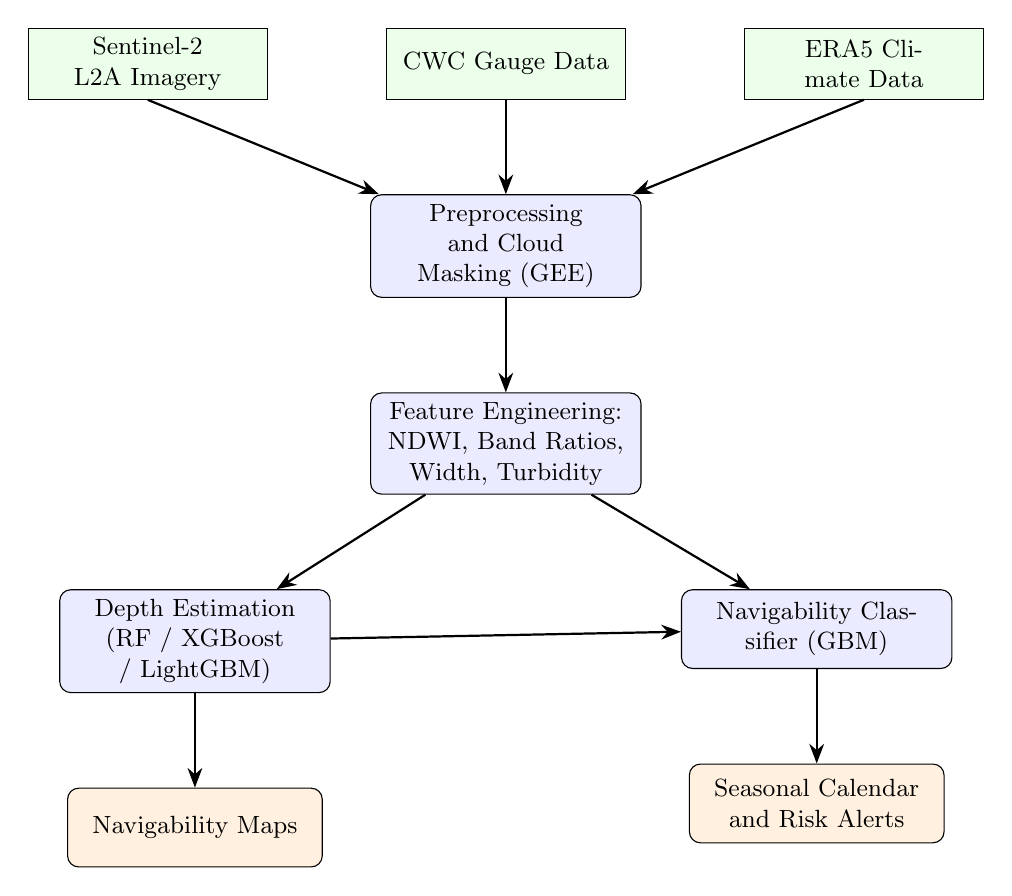
\begin{tikzpicture}[
    node distance=1.2cm and 0.3cm,
    block/.style={rectangle, draw, fill=blue!8, text width=3.2cm, text centered, rounded corners, minimum height=1cm, font=\small},
    data/.style={rectangle, draw, fill=green!8, text width=2.8cm, text centered, minimum height=0.9cm, font=\small},
    output/.style={rectangle, draw, fill=orange!12, text width=3cm, text centered, rounded corners, minimum height=1cm, font=\small},
    arrow/.style={-{Stealth[length=2.5mm]}, thick}
]

% Data sources
\node[data] (s2) {Sentinel-2 L2A Imagery};
\node[data, right=1.5cm of s2] (cwc) {CWC Gauge Data};
\node[data, right=1.5cm of cwc] (era5) {ERA5 Climate Data};

% Preprocessing
\node[block, below=1.2cm of cwc] (preproc) {Preprocessing and Cloud Masking (GEE)};

% Feature Engineering
\node[block, below=1.2cm of preproc] (feat) {Feature Engineering: NDWI, Band Ratios, Width, Turbidity};

% Models
\node[block, below left=1.2cm and 0.5cm of feat] (depth) {Depth Estimation (RF / XGBoost / LightGBM)};
\node[block, below right=1.2cm and 0.5cm of feat] (nav) {Navigability Classifier (GBM)};

% Outputs
\node[output, below=1.2cm of depth] (map) {Navigability Maps};
\node[output, below=1.2cm of nav] (cal) {Seasonal Calendar and Risk Alerts};

% Arrows
\draw[arrow] (s2.south) -- (preproc);
\draw[arrow] (cwc.south) -- (preproc);
\draw[arrow] (era5.south) -- (preproc);
\draw[arrow] (preproc) -- (feat);
\draw[arrow] (feat) -- (depth);
\draw[arrow] (feat) -- (nav);
\draw[arrow] (depth) -- (nav);
\draw[arrow] (depth) -- (map);
\draw[arrow] (nav) -- (cal);

\end{tikzpicture}
\caption{System architecture showing data flow from satellite and hydrological sources through preprocessing, feature engineering, and machine learning models to navigability outputs.}
\label{fig:architecture}
\end{figure}

\vspace{0.3cm}
\noindent\textbf{Validation Strategy}

Model outputs will be validated at three levels:

\begin{enumerate}[leftmargin=1.5cm]
\item \textbf{Point validation:} Predicted depth values compared against held-out CWC gauge readings (20\% of gauge data reserved for testing, split by spatial blocks).
\item \textbf{Segment validation:} Navigability classifications compared against IWAI monthly LAD bulletins for NW-1 segments where survey data is available.
\item \textbf{Temporal validation:} The model trained on data from 2019 to 2023 will be evaluated on 2024 data (out-of-sample temporal generalisation).
\end{enumerate}

\newpage
\subsection*{3.2 Time Schedule of Activities Giving Milestones through BAR Diagram}

The project timeline spans 18 months (1.5 years), divided into six work packages. Table~\ref{tab:milestones} summarises the milestones, and the Gantt chart in Figure~\ref{fig:gantt} illustrates the schedule.

\begin{table}[H]
\centering
\caption{Work packages and milestones.}
\label{tab:milestones}
\begin{tabular}{c p{5.5cm} c p{4.5cm}}
\toprule
\textbf{WP} & \textbf{Activity} & \textbf{Duration} & \textbf{Milestone / Deliverable} \\
\midrule
1 & Literature survey and study area finalisation & Months 1--3 & Review report and study area maps \\
2 & Data acquisition and preprocessing pipeline & Months 3--6 & Clean multi-year Sentinel-2 archive on GEE \\
3 & Feature engineering and exploratory data analysis & Months 5--8 & Feature matrix, EDA report \\
4 & Model training, tuning, and benchmarking & Months 7--12 & Depth model with $R^{2} > 0.85$ on NW-1 \\
5 & Navigability classification and visualisation & Months 10--14 & Interactive navigability maps and calendar \\
6 & Validation, documentation, and paper writing & Months 13--18 & Final report and research manuscript \\
\bottomrule
\end{tabular}
\end{table}

\begin{figure}[H]
\centering
\begin{ganttchart}[
    hgrid,
    vgrid={*{17}{dotted}, solid},
    x unit=0.55cm,
    y unit chart=0.7cm,
    title height=1,
    bar height=0.6,
    bar label font=\small,
    title label font=\small,
    milestone label font=\small,
    group label font=\small\bfseries,
    bar/.append style={fill=blue!25},
    milestone/.append style={fill=red!60},
]{1}{18}

\gantttitle{Project Timeline (Months)}{18} \\
\gantttitlelist{1,...,18}{1} \\

\ganttbar{WP1: Literature Survey}{1}{3} \\
\ganttbar{WP2: Data Acquisition}{3}{6} \\
\ganttbar{WP3: Feature Engineering}{5}{8} \\
\ganttbar{WP4: Model Development}{7}{12} \\
\ganttbar{WP5: Classification and Maps}{10}{14} \\
\ganttbar{WP6: Validation and Report}{13}{18} \\

\ganttmilestone{M1: Study area finalised}{3} \\
\ganttmilestone{M2: Data pipeline operational}{6} \\
\ganttmilestone{M3: Depth model benchmarked}{12} \\
\ganttmilestone{M4: Final report submitted}{18}

\end{ganttchart}
\caption{Gantt chart with milestones for the 18-month project period.}
\label{fig:gantt}
\end{figure}

\vspace{1cm}

%==============================================================
\section*{References}
%==============================================================

\begin{enumerate}[leftmargin=0.7cm, label={[\arabic*]}]
\item Lyzenga, D.R. (1985). Shallow-water bathymetry using combined lidar and passive multispectral scanner data. \textit{International Journal of Remote Sensing}, 6(1), 115--125.
\item Stumpf, R.P., Holderied, K., and Sinclair, M. (2003). Determination of water depth with high-resolution satellite imagery over variable bottom types. \textit{Limnology and Oceanography}, 48(1), 547--556.
\item McFeeters, S.K. (1996). The use of the Normalized Difference Water Index (NDWI) in the delineation of open water features. \textit{International Journal of Remote Sensing}, 17(7), 1425--1432.
\item Xu, H. (2006). Modification of normalised difference water index (NDWI) to enhance open water features in remotely sensed imagery. \textit{International Journal of Remote Sensing}, 27(14), 3025--3033.
\item Li, J. \textit{et al.} (2023). Comparison of machine learning and empirical models for satellite-derived bathymetry. \textit{Remote Sensing}, 15(4), 1012.
\item Hassan, M.A. \textit{et al.} (2023). Fine decision tree regression for river depth estimation from multispectral satellite images. \textit{Egyptian Journal of Remote Sensing and Space Sciences}, 26(2), 300--312.
\item Zhang, W. \textit{et al.} (2025). Spectral-geospatial XGBoost for turbid water bathymetry. Preprint, SkyBathy.
\item Caballero, I. and Stumpf, R.P. (2020). Towards routine coastline monitoring with Sentinel-2. \textit{Remote Sensing of Environment}, 236, 111468.
\item Chen, Y. \textit{et al.} (2023). Long-term river width dynamics from Sentinel-2 MNDWI time series in the Aral Sea Basin. \textit{E3S Web of Conferences}, 401, 01023.
\item Papa, F. \textit{et al.} (2022). Multi-mission altimetry to evaluate hydrodynamic models on the Mahanadi River, India. \textit{Hydrology and Earth System Sciences}, 26, 1897--1912.
\item Dubey, A.K. \textit{et al.} (2020). Satellite altimetry for inland water body monitoring over the Indian subcontinent. \textit{Journal of the Indian Society of Remote Sensing}, 48(5), 767--780.
\item Sarkar, A. \textit{et al.} (2021). Multi-decadal channel planform dynamics of the Brahmaputra River from Landsat imagery. \textit{Geomorphology}, 389, 107840.
\item Gupta, R. and Rajan, K.S. (2022). Multi-sensor fusion for river monitoring through cloud-covered monsoon months. \textit{IEEE Journal of Selected Topics in Applied Earth Observations}, 15, 4521--4533.
\item Ministry of Ports, Shipping and Waterways, Government of India (2025). Inland Waterways Cargo Achievement Report, FY 2024--25. Press Information Bureau.
\item IWAI (2024). National Waterways Development Status Report. Inland Waterways Authority of India.
\end{enumerate}

\end{document}
